\documentclass[a4paper,12pt]{article}

\usepackage[ngerman]{babel}
\usepackage[T1]{fontenc}
\usepackage{amsmath}
\usepackage{graphicx}
\usepackage{hyperref}
\usepackage[
backend=biber,
style=ieee,
citestyle=numeric
]{biblatex}
\usepackage{placeins}


\addbibresource{literature.bib}

\title{YOLOv8 Algorithmus und seine Verbesserungen im Vergleich zu früheren Versionen}
\author{Benjamin Albrecht}
\date{\today}

\begin{document}

\sloppy
\maketitle
\tableofcontents

\section{Aufbau und Funktionsweise des Algorithmus}
\subsection{YOLOv8 und frühere Versionen}
Die Verbesserungen in YOLOv8 im Vergleich zu früheren Versionen beziehen sich auf die Non-Maximum Suppression, Anchor-Free Strategies und Loss Functions.\par\vspace{0.5em}

\noindent Non-Maximum Suppression (NMS) ist ein Verfahren, mit dem die Anzahl der überlappender Bounding Boxes reduziert wird. Denn dies wählt die beste Bounding Box aus einer Gruppe überlappender Boxen aus. Ist eine Bounding Box unter einer besimmten Konfidenzschwelle, wird diese verworfen. Verbleibende Bounding Boxes werden nach ihren Konfidenzwerten sortiert. In frühere Versionen wurde das klassische NMS verwendet, bei dem eine Box mit dem höchsten Konfidenzwert beibehalten und andere Boxen, die stark überlappen (über einem bestimmten IoU-Schwellenwert), verworfen werden.\par\vspace{0.5em}

\noindent YOLO basiert in früheren Versionen auf vordefinierte Ankerboxen. YOLOv8 hingegen nicht, denn hier werden ankerfreier Mechanismen verwendet, um flexibler auf unterschiedliche Objekte zu reagieren. Dies erspart ebenfalls den Vorverarbeitungsaufwand für das Definieren von Ankerboxen.\par\vspace{0.5em}
\noindent Der Loss Function misst die Differenz zwischen den vorhergesagten Ausgaben des Modells und die tatsächlichen Labels in den Trainingsdaten und versucht diese zu minimieren. In YOLOv8 wurde dieser verbessert mit dem Ziel eine höhere Genauigkeit von Objekten zu erreichen \cite{terven2023comprehensive, reis2023real, safaldin2024improved}.\par\vspace{0.5em}


\section{Mathematischer Hintergrund / Mechanismen im Hintergrund}
\subsection{Non-Maximum Suppression}

\noindent In YOLOv8 kommt der Efficient-IoU in Einsatz, wenn es um das Behandeln von Bounding Boxes geht. Und es wurde eine weiche Strategie aus Soft-NMS angenommen, um die Confidence Scores der überlappenden Boxes zu verringern, anstatt sie zu verwerfen. Denn dieser Einsatz ermöglicht die Erhaltung von mehr Bounding Boxes, die überlappende Objekte enthalten. Des Weiteren wird der verbesserte Algorithmus zur Vereinfachung als E-Soft-NMS bezeichnet.

\noindent Der E-Soft-NMS wird wie folgt berechnet:

\begin{figure}[h]
    \centering
    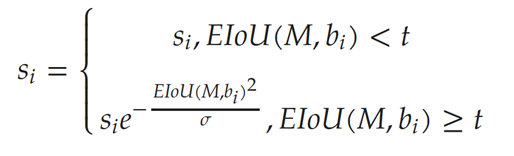
\includegraphics[width=\textwidth, height=\textheight, keepaspectratio]{Bild1.png}
    \caption{E-Soft-NMS Formel}
    \label{fig:bild1}
\end{figure}

\noindent $S_i$ steht für den Confidence Score. $M$ für die Box mit maximalem Confidence Score. $b_i$ steht für die andere Bounding Box und $t$ ist der Schwellenwert. Überschreitet der $EIoU$-Wert zwischen $b_i$ und $M$ den Schwellenwert, soll die Punktzahl von $b_i$ mit der Abnahmefunktion multipliziert werden. Wenn nur der Confidence Score gesenkt wird, können redundante Boxes, die dasselbe Ziel vorhersagen, vorhanden sein. Um ihre Entfernung zu verhindern, wird eine Gaußsche Abnahmefunktion verwendet, die mit $EIoU$ zusammenhängt. Detektionsrahmen, die weit von $M$ entfernt sind, sind nicht betroffen, während solche, die sich nahe bei $M$ befinden, stärker bestraft werden. Somit werden Boxes, die unterschiedliche Ziele vorhersagen, erhalten bleiben, redundante Rahmen, die dasselbe Ziel vorhersagen, jedoch entfernt.

\noindent Die Formel für die Gaußsche Abnahmefunktion lautet:

\begin{figure}[h]
    \centering
    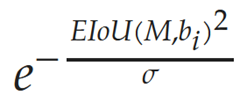
\includegraphics[width=0.3\textwidth, height=\textheight, keepaspectratio]{Bild2.png}
    \caption{Gaußsche Abnahmefunktion}
    \label{fig:bild2}
\end{figure}

\noindent Und für die EIoU-Berechnung:

\begin{figure}[h]
    \centering
    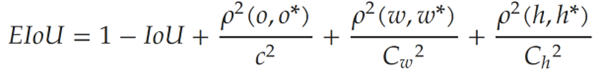
\includegraphics[width=0.8\textwidth, height=\textheight, keepaspectratio]{Bild3.png}
    \caption{EIoU-Berechnung}
    \label{fig:bild3}
\end{figure}

\noindent Wobei $\mathbf{o}$ für das Zentrum von $b_i$, $o^*$ für das Zentrum von $M$, $p$ für den euklidischen Abstand zwischen $\mathbf{o}$ und $o^*$ stehen. $w$ und $w^*$ in die Breiten von $b_i$ und $M$. $h$ und $h^*$ sind die Höhen von $b_i$ und $M$. $c$ ist die diagonale Länge der minimalen Box $B$, der $b_i$ und $M$ umschließt. Die Breite und Höhe $B$ sind $C_w$ und $C_h$ \cite{han2023improving}.

\subsection{Anchor-Free Strategies}
Im Rahmen des ankerfreien Mechanismus von FCOS stellt die folgende Formel die Basis dar, da sie Abstände eines Rasterpunkts zu den Rändern der Bounding Box beschreibt, was eine präzise und flexible Objekterkennung ermöglicht, ohne auf vordefinierte Ankerboxen angewiesen zu sein \cite{tian2019fcos, wang2018anchor}.

\begin{figure}[h]
    \centering
    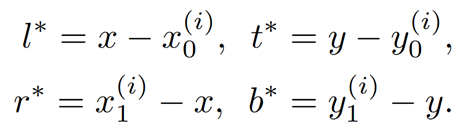
\includegraphics[width=0.6\textwidth, height=\textheight, keepaspectratio]{Bild4.png}
    \caption{Anchor-Free Strategies}
    \label{fig:bild4}
\end{figure}



\noindent $x$ und $y$ stehen für die Koordinaten des Punktes auf dem Feature-Grid, der als Zentrum der Bounding Box verwendet wird. $x_0^{(i)}$ und $y_0^{(i)}$ sind die Koordinaten des oberen linken Eckpunkts der Ground Truth Bounding Box $i$. $l^*$ steht für den horizontalen Abstand vom Punkt $(x,y)$ zur linken Grenze der Bounding Box. $t^*$ steht für den vertikalen Abstand vom Punkt $(x,y)$ zur oberen Grenze der Bounding Box. Für den horizontalen Abstand vom Punkt $(x,y)$ zur rechten Grenze der Bounding Box steht $r^*$. Und $b^*$ für den vertikalen Abstand vom Punkt $(x,y)$ zur unteren Grenze der Bounding Box.
Das bedeutet, dass anstatt feste Ankerboxen zu verwenden, die Bounding Box durch die Berechnung dieser Distanzen relativ zu einem Punkt auf dem Grid bestimmt wird \cite{tian2019fcos, wang2018anchor}.

\subsection{Loss Calculation}
Die zwei Teile, aus denen der Verlustberechnungsprozess besteht, sind die Stichprobenzuweisungsstrategie und die Verlustberechnung. In modernen Detektoren werden dynamische Stichprobenzuweisungsstrategien wie simOTA von YOLOX, TaskAlignedAssigner von TOOD und DynamicSoftLAvelAssigner von RTMDet verwendet. Der YOLOv8-Algorithmus integriert die in TaskAlignedAssigner von TOOD verwendete Strategie direkt \cite{openmmlab2023dive}.

\noindent Zusammengefasst kann die Matching-Strategie von TaskAlignedAssigner mit einfachen Termen beschrieben werden. Die positiven Stichproben werden basierend auf den gewichteten Bewertungen von Klassifizierung und Regression ausgewählt.

\begin{figure}[h]
    \centering
    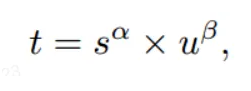
\includegraphics[width=0.3\textwidth]{Bild5.png}
    \caption{Loss Calculation}
    \label{fig:bild5}
\end{figure}

\noindent wobei $s$ die Vorhersagebewertung ist, die der Ground-Truth-Kategorie entspricht. $u$ ist die Intersection Over Union (IoU) des Vorhersage-Bounding Boxes und des Ground Truth (gt)-Bounding Boxes.

\noindent Der Task-Aligned-Assigner berechnet für jede Ground Truth die Alignment-Metrik für jeden Anker, indem er das gewichtete Produkt zweier Werte nimmt: den vorhergesagten Klassifizierungswert der entsprechenden Klasse und die IoU zwischen der vorhergesagten Begrenzungsbox und der Ground Truth-Begrenzungsbox.

\noindent Es werden für jede Ground Truth die größten Top-k-Samples direkt auf der Grundlage der Alignment\_metrics-Werte als positiv ausgewählt. Die Verlustberechnung besteht aus der Klassifizierung und der Regression, ohne den „Objectness Loss“ im vorherigen Modell \cite{openmmlab2023dive}.


\section{Architektur von YOLOv8}
YOLOv8 besteht aus einer strukturierten Reihe von Convolutional Neural Networks (CNNs) mit den die Lokalisierung und Klassifizierung von Objekten ermöglicht wird. Die Hauptkomponente der Architektur sind Backbone, Neck und Head.


\begin{itemize}
    \item \textbf{Backbone}: Ein tiefes CNN, das als Feature-Extraktor dient. Wesentliche Merkmale aus dem Eingabebild werden hiermit extrahiert.
    \item \textbf{Neck}: Verarbeitet die extrahierten Merkmale und kombiniert die Informationen, um sie an den Head weiterzugeben.
    \item \textbf{Head}: Empfängt die extrahierten Merkmale und die kombinierten Informationen und gibt Bounding Boxes und Class Scores für jedes erkannte Objekt aus.
\end{itemize}

\FloatBarrier
\begin{figure}[h]
    \centering
    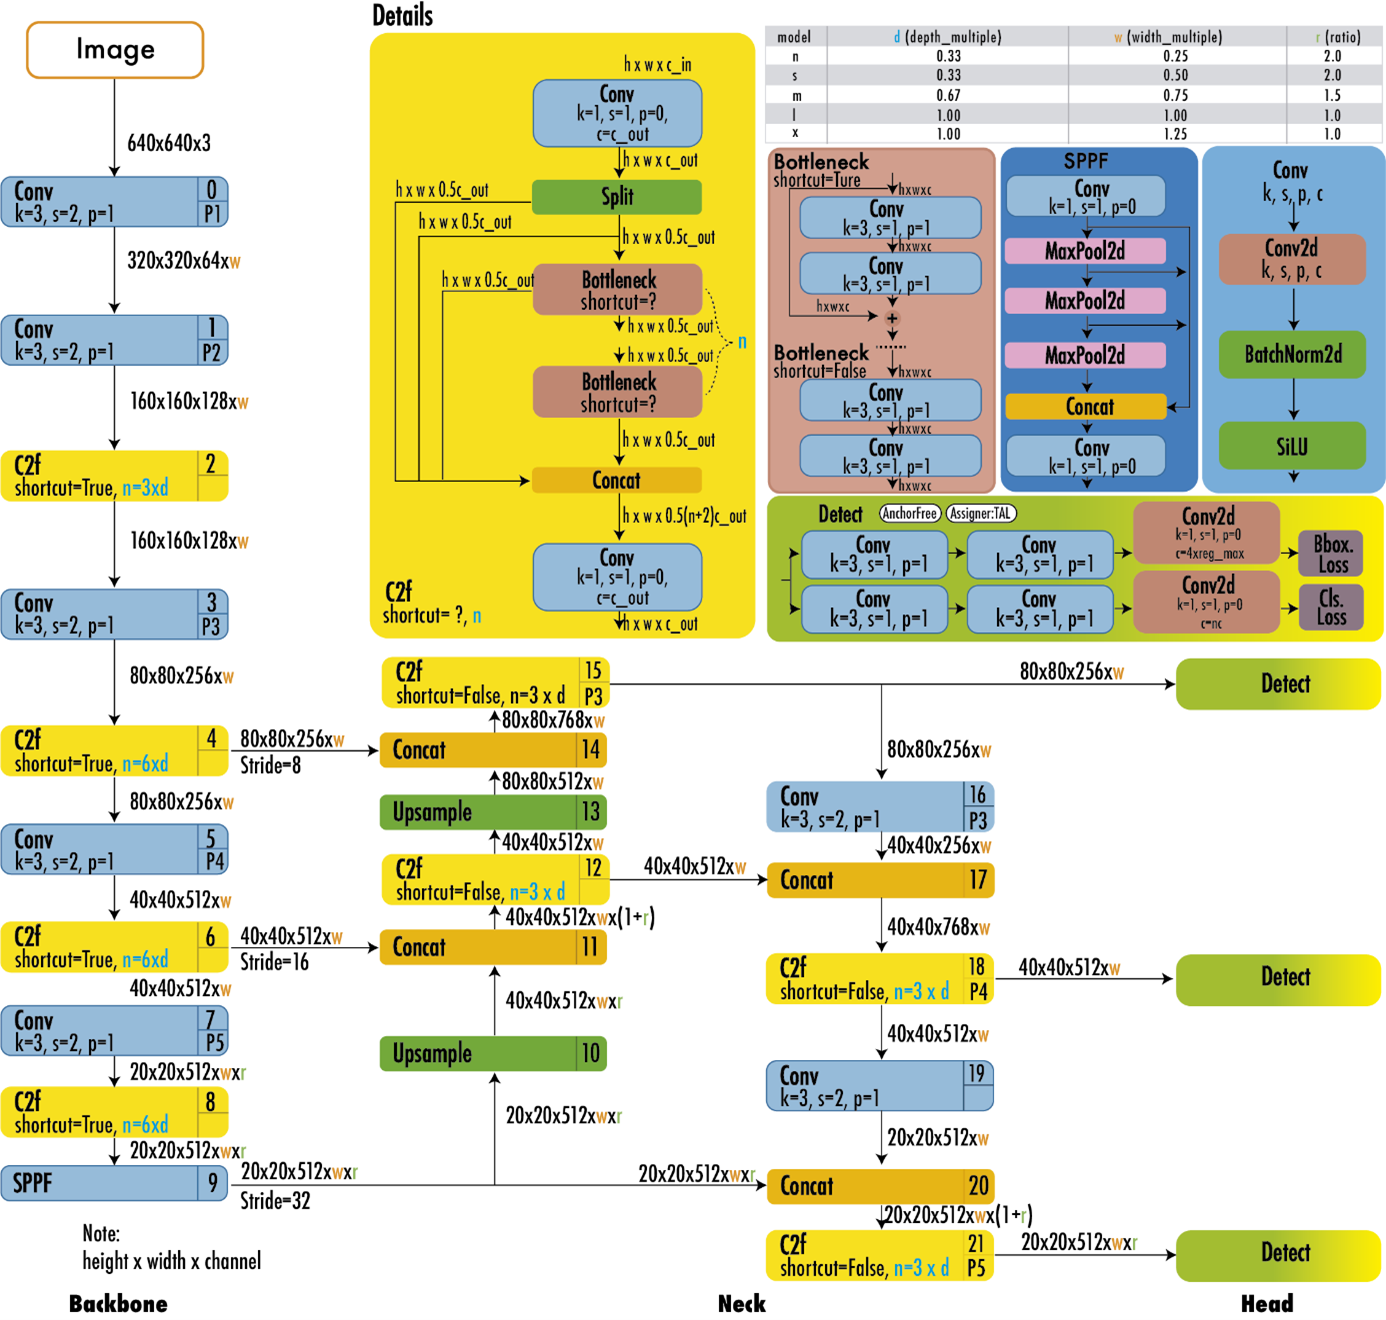
\includegraphics[width=\textwidth]{Bild6.png}
    \caption{YOLOv8 Architektur}
    \label{fig:bild6}
\end{figure}
\FloatBarrier

\noindent Der meistgenutzte Block ist der Convolutional Block. Dieser besteht aus 2D-Convolutional Layer, 2D-Batch Normalization und einer SiLU-Aktivierungsfunktion. 

\noindent Die Tabelle in der Abbildung [Nils muss hier die Nummer der Abbildung einfügen] enthält Modellgröße, -tiefe, -breite und -verhältnis. Es lässt sich bemerken, dass die Tiefe des Modells bei höheren Modellgrößen steigt. Dies gilt ebenfalls für die Tiefe. Jedoch sinkt das Skalierungsverhältnis bei steigenden Modellgrößen, da größere Modelle bereits höhere Tiefe- und Breitewerte haben und somit von Natur aus tiefer und breiter sind. Zusätzliche Skalierung könnte zu hohem Rechenaufwand führen \cite{terven2023comprehensive}.

\noindent 

\FloatBarrier

\printbibliography

\end{document}